\documentclass{standalone}
\usepackage{tikz}
\usetikzlibrary{patterns, positioning}


\begin{document}
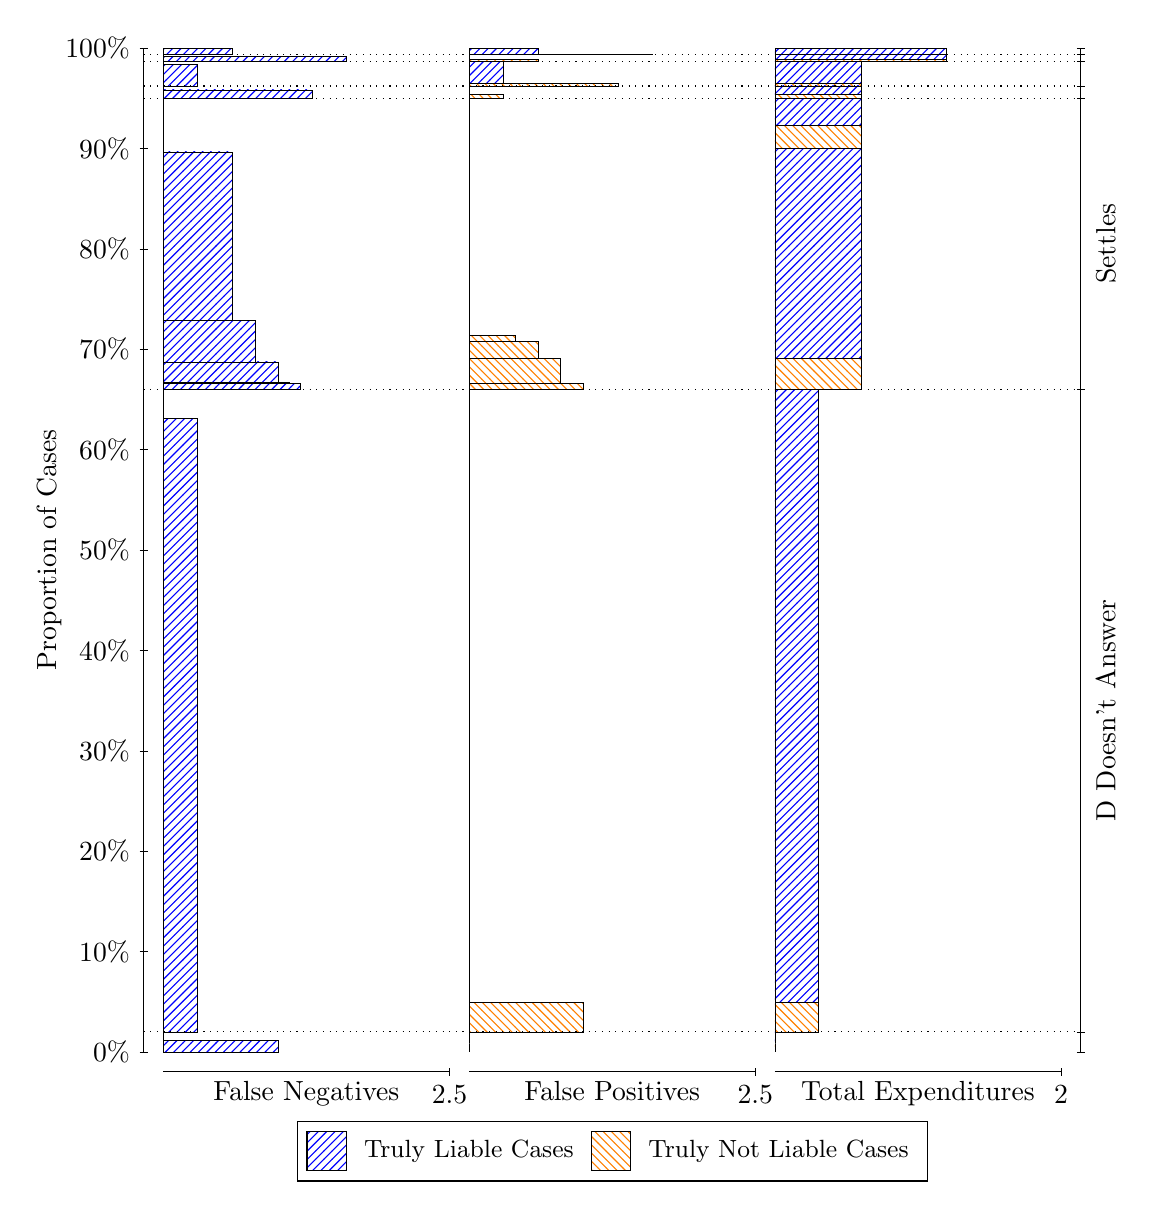
\begin{tikzpicture}
\draw[black, very thin] (1.5,1.75) -- (1.5,14.5);
\node[rotate=90, text=black, anchor=center] at (0.3, 8.125) {Proportion of Cases};
\draw[black, very thin] (1.45,1.75) -- (1.55,1.75);
\node[text=black, anchor=east] at (1.45, 1.75) {0\%};
\draw[black, very thin] (1.45,3.025) -- (1.55,3.025);
\node[text=black, anchor=east] at (1.45, 3.025) {10\%};
\draw[black, very thin] (1.45,4.3) -- (1.55,4.3);
\node[text=black, anchor=east] at (1.45, 4.3) {20\%};
\draw[black, very thin] (1.45,5.575) -- (1.55,5.575);
\node[text=black, anchor=east] at (1.45, 5.575) {30\%};
\draw[black, very thin] (1.45,6.85) -- (1.55,6.85);
\node[text=black, anchor=east] at (1.45, 6.85) {40\%};
\draw[black, very thin] (1.45,8.125) -- (1.55,8.125);
\node[text=black, anchor=east] at (1.45, 8.125) {50\%};
\draw[black, very thin] (1.45,9.4) -- (1.55,9.4);
\node[text=black, anchor=east] at (1.45, 9.4) {60\%};
\draw[black, very thin] (1.45,10.675) -- (1.55,10.675);
\node[text=black, anchor=east] at (1.45, 10.675) {70\%};
\draw[black, very thin] (1.45,11.95) -- (1.55,11.95);
\node[text=black, anchor=east] at (1.45, 11.95) {80\%};
\draw[black, very thin] (1.45,13.225) -- (1.55,13.225);
\node[text=black, anchor=east] at (1.45, 13.225) {90\%};
\draw[black, very thin] (1.45,14.5) -- (1.55,14.5);
\node[text=black, anchor=east] at (1.45, 14.5) {100\%};

\draw[black, very thin] (13.4,1.75) -- (13.4,14.5);
\draw[black, very thin] (13.35,1.75) -- (13.45,1.75);
\node[anchor=west] at (13.35, 1.75) {};
\draw[black, very thin] (13.35,2.0047) -- (13.45,2.0047);
\node[anchor=west] at (13.35, 2.0047) {};
\draw[black, very thin] (13.35,10.167) -- (13.45,10.167);
\node[anchor=west] at (13.35, 10.167) {};
\draw[black, very thin] (13.35,13.863) -- (13.45,13.863);
\node[anchor=west] at (13.35, 13.863) {};
\draw[black, very thin] (13.35,14.018) -- (13.45,14.018);
\node[anchor=west] at (13.35, 14.018) {};
\draw[black, very thin] (13.35,14.329) -- (13.45,14.329);
\node[anchor=west] at (13.35, 14.329) {};
\draw[black, very thin] (13.35,14.417) -- (13.45,14.417);
\node[anchor=west] at (13.35, 14.417) {};
\draw[black, very thin] (13.35,14.5) -- (13.45,14.5);
\node[anchor=west] at (13.35, 14.5) {};

\draw[black, very thin, pattern color=blue, pattern=north east lines] (1.75,1.75) rectangle (3.2033,1.894);
\draw[black, very thin, pattern color=orange, pattern=north west lines] (1.75,1.894) rectangle (1.75,2.0047);
\draw[black, very thin, pattern color=blue, pattern=north east lines] (1.75,2.0047) rectangle (2.186,9.7963);
\draw[black, very thin, pattern color=orange, pattern=north west lines] (1.75,9.7963) rectangle (1.75,10.167);
\draw[black, very thin, pattern color=blue, pattern=north east lines] (1.75,10.167) rectangle (3.494,10.244);
\draw[black, very thin, pattern color=blue, pattern=north east lines] (1.75,10.244) rectangle (3.3487,10.254);
\draw[black, very thin, pattern color=blue, pattern=north east lines] (1.75,10.254) rectangle (3.2033,10.513);
\draw[black, very thin, pattern color=blue, pattern=north east lines] (1.75,10.513) rectangle (2.9127,11.042);
\draw[black, very thin, pattern color=blue, pattern=north east lines] (1.75,11.042) rectangle (2.622,13.181);
\draw[black, very thin, pattern color=orange, pattern=north west lines] (1.75,13.181) rectangle (1.75,13.863);
\draw[black, very thin, pattern color=blue, pattern=north east lines] (1.75,13.863) rectangle (3.6393,13.969);
\draw[black, very thin, pattern color=orange, pattern=north west lines] (1.75,13.969) rectangle (1.75,14.018);
\draw[black, very thin, pattern color=blue, pattern=north east lines] (1.75,14.018) rectangle (2.186,14.297);
\draw[black, very thin, pattern color=orange, pattern=north west lines] (1.75,14.297) rectangle (1.75,14.329);
\draw[black, very thin, pattern color=blue, pattern=north east lines] (1.75,14.329) rectangle (4.0753,14.393);
\draw[black, very thin, pattern color=orange, pattern=north west lines] (1.75,14.393) rectangle (1.75,14.417);
\draw[black, very thin, pattern color=blue, pattern=north east lines] (1.75,14.417) rectangle (2.622,14.493);
\draw[black, very thin, pattern color=orange, pattern=north west lines] (1.75,14.493) rectangle (1.75,14.5);
\draw[black, very thin, pattern color=orange, pattern=north west lines] (5.6333,1.75) rectangle (5.6333,1.8607);
\draw[black, very thin, pattern color=blue, pattern=north east lines] (5.6333,1.8607) rectangle (5.6333,2.0047);
\draw[black, very thin, pattern color=orange, pattern=north west lines] (5.6333,2.0047) rectangle (7.0867,2.3749);
\draw[black, very thin, pattern color=blue, pattern=north east lines] (5.6333,2.3749) rectangle (5.6333,10.167);
\draw[black, very thin, pattern color=orange, pattern=north west lines] (5.6333,10.167) rectangle (7.0867,10.245);
\draw[black, very thin, pattern color=orange, pattern=north west lines] (5.6333,10.245) rectangle (6.796,10.559);
\draw[black, very thin, pattern color=orange, pattern=north west lines] (5.6333,10.559) rectangle (6.5053,10.77);
\draw[black, very thin, pattern color=orange, pattern=north west lines] (5.6333,10.77) rectangle (6.36,10.777);
\draw[black, very thin, pattern color=orange, pattern=north west lines] (5.6333,10.777) rectangle (6.2147,10.849);
\draw[black, very thin, pattern color=blue, pattern=north east lines] (5.6333,10.849) rectangle (5.6333,13.863);
\draw[black, very thin, pattern color=orange, pattern=north west lines] (5.6333,13.863) rectangle (6.0693,13.912);
\draw[black, very thin, pattern color=blue, pattern=north east lines] (5.6333,13.912) rectangle (5.6333,14.018);
\draw[black, very thin, pattern color=orange, pattern=north west lines] (5.6333,14.018) rectangle (7.5227,14.05);
\draw[black, very thin, pattern color=blue, pattern=north east lines] (5.6333,14.05) rectangle (6.0693,14.329);
\draw[black, very thin, pattern color=orange, pattern=north west lines] (5.6333,14.329) rectangle (6.5053,14.353);
\draw[black, very thin, pattern color=blue, pattern=north east lines] (5.6333,14.353) rectangle (5.6333,14.417);
\draw[black, very thin, pattern color=orange, pattern=north west lines] (5.6333,14.417) rectangle (7.9587,14.424);
\draw[black, very thin, pattern color=blue, pattern=north east lines] (5.6333,14.424) rectangle (6.5053,14.5);
\draw[black, very thin, pattern color=orange, pattern=north west lines] (9.5167,1.75) rectangle (9.5167,1.8607);
\draw[black, very thin, pattern color=blue, pattern=north east lines] (9.5167,1.8607) rectangle (9.5167,2.0047);
\draw[black, very thin, pattern color=orange, pattern=north west lines] (9.5167,2.0047) rectangle (10.062,2.3749);
\draw[black, very thin, pattern color=blue, pattern=north east lines] (9.5167,2.3749) rectangle (10.062,10.167);
\draw[black, very thin, pattern color=orange, pattern=north west lines] (9.5167,10.167) rectangle (10.607,10.559);
\draw[black, very thin, pattern color=blue, pattern=north east lines] (9.5167,10.559) rectangle (10.607,13.227);
\draw[black, very thin, pattern color=orange, pattern=north west lines] (9.5167,13.227) rectangle (10.607,13.517);
\draw[black, very thin, pattern color=blue, pattern=north east lines] (9.5167,13.517) rectangle (10.607,13.863);
\draw[black, very thin, pattern color=orange, pattern=north west lines] (9.5167,13.863) rectangle (10.607,13.912);
\draw[black, very thin, pattern color=blue, pattern=north east lines] (9.5167,13.912) rectangle (10.607,14.018);
\draw[black, very thin, pattern color=orange, pattern=north west lines] (9.5167,14.018) rectangle (10.607,14.05);
\draw[black, very thin, pattern color=blue, pattern=north east lines] (9.5167,14.05) rectangle (10.607,14.329);
\draw[black, very thin, pattern color=orange, pattern=north west lines] (9.5167,14.329) rectangle (11.697,14.353);
\draw[black, very thin, pattern color=blue, pattern=north east lines] (9.5167,14.353) rectangle (11.697,14.417);
\draw[black, very thin, pattern color=orange, pattern=north west lines] (9.5167,14.417) rectangle (11.697,14.424);
\draw[black, very thin, pattern color=blue, pattern=north east lines] (9.5167,14.424) rectangle (11.697,14.5);
\draw[black, dotted] (1.5,2.0047) -- (13.4,2.0047);
\draw[black, dotted] (1.5,10.167) -- (13.4,10.167);
\draw[black, dotted] (1.5,13.863) -- (13.4,13.863);
\draw[black, dotted] (1.5,14.018) -- (13.4,14.018);
\draw[black, dotted] (1.5,14.329) -- (13.4,14.329);
\draw[black, dotted] (1.5,14.417) -- (13.4,14.417);
\draw[black, very thin] (1.75,1.5) -- (5.3833,1.5);
\node[text=black, anchor=north] at (3.5667, 1.5) {False Negatives};
\draw[black, very thin] (5.3833,1.45) -- (5.3833,1.55);
\node[text=black, anchor=north] at (5.3833, 1.45) {2.5};

\draw[black, very thin] (5.6333,1.5) -- (9.2667,1.5);
\node[text=black, anchor=north] at (7.45, 1.5) {False Positives};
\draw[black, very thin] (9.2667,1.45) -- (9.2667,1.55);
\node[text=black, anchor=north] at (9.2667, 1.45) {2.5};

\draw[black, very thin] (9.5167,1.5) -- (13.15,1.5);
\node[text=black, anchor=north] at (11.333, 1.5) {Total Expenditures};
\draw[black, very thin] (13.15,1.45) -- (13.15,1.55);
\node[text=black, anchor=north] at (13.15, 1.45) {2};


\node[text=black, centered, rotate=90] at (13.72, 6.0856) {D Doesn't Answer};
\node[text=black, centered, rotate=90] at (13.72, 12.015) {Settles};





\draw (7.449999999999999,1.5) node[draw=none] (baseCoordinate) {};
\begin{scope}[align=center]
        \matrix[scale=0.5, draw=black, below=0.5cm of baseCoordinate, nodes={draw}, column sep=0.1cm]{
            \node[rectangle, draw, minimum width=0.5cm, minimum height=0.5cm, pattern color=blue, pattern=north east lines] {}; &
            \node[draw=none, font=\small, text=black] (B) {Truly Liable Cases}; &
            \node[rectangle, draw, minimum width=0.5cm, minimum height=0.5cm, pattern color=orange, pattern=north west lines] {}; &
            \node[draw=none, font=\small, text=black] (B) {Truly Not Liable Cases}; \\
            };
\end{scope}

\end{tikzpicture}
\end{document}